% ============================================================
%  Re-evaluating the Sun Liu Alliance in the Battle of Red Cliffs
%  A Digital Humanities Research Report
%  LaTeX Source. Compiled with pdflatex (or lualatex)
% ============================================================

\documentclass[12pt, a4paper]{article}
\usepackage{hyphenat}
% ── Packages ────────────────────────────────────────────────
\usepackage[T1]{fontenc}
\usepackage[utf8]{inputenc}
\usepackage{lmodern}
\usepackage[margin=2.54cm]{geometry}
\usepackage{setspace}
\usepackage{microtype}
\usepackage{parskip}          % blank line between paragraphs, no indent
\usepackage{titlesec}
\usepackage{titling}
\usepackage{abstract}
\usepackage{booktabs}
\usepackage{tabularx}
\usepackage{array}
\usepackage{longtable}
\usepackage{graphicx}
\usepackage{float}
\usepackage{caption}
\usepackage{subcaption}
\usepackage{listings}
\usepackage{xcolor}
\usepackage{hyperref}
\usepackage{url}
\usepackage{enumitem}
\usepackage{amsmath}
\usepackage{csquotes}
\usepackage[style=authoryear, backend=biber]{biblatex}

% ── Bibliography ─────────────────────────────────────────────
\addbibresource{references.bib}

% ── Typography & Spacing ─────────────────────────────────────
\onehalfspacing
\setlength{\parskip}{6pt}

% ── Section title formatting ─────────────────────────────────
\titleformat{\section}{\large\bfseries}{\thesection.}{0.6em}{}
\titleformat{\subsection}{\normalsize\bfseries}{\thesubsection.}{0.6em}{}
\titleformat{\subsubsection}{\normalsize\itshape}{\thesubsubsection.}{0.6em}{}

% ── Code listing style ───────────────────────────────────────
\definecolor{codebg}{HTML}{F5F5F5}
\definecolor{codeframe}{HTML}{CCCCCC}
\definecolor{codecomment}{HTML}{5C8A3F}
\definecolor{codestring}{HTML}{A31515}
\definecolor{codekeyword}{HTML}{0000CD}

\lstdefinelanguage{R}{
  keywords={library, mutate, filter, select, arrange, group_by,
            summarise, left_join, as_tbl_graph, tbl_graph,
            ggraph, geom_edge_link, geom_node_point,
            geom_node_text, aes, scale_color_gradient2,
            scale_edge_width, st_read, st_transform,
            st_coordinates, st_as_sf, ggplot, geom_sf,
            geom_point, geom_path, labs, theme_minimal,
            centrality_eigen, centrality_degree,
            theme, element_text, coord_sf, facet_wrap},
  sensitive=true,
  comment=[l]{\#},
  morestring=[b]",
  morestring=[b]'
}

\lstset{
  language=R,
  backgroundcolor=\color{codebg},
  frame=single,
  rulecolor=\color{codeframe},
  basicstyle=\ttfamily\small,
  keywordstyle=\color{codekeyword}\bfseries,
  commentstyle=\color{codecomment}\itshape,
  stringstyle=\color{codestring},
  breaklines=true,
  showstringspaces=false,
  numbers=left,
  numberstyle=\tiny\color{gray},
  numbersep=5pt,
  xleftmargin=12pt,
  captionpos=b
}

% ── Hyperref ─────────────────────────────────────────────────
\hypersetup{
  colorlinks=true,
  linkcolor=black,
  citecolor=black,
  urlcolor=blue,
  pdftitle={Re-evaluating the Sun Liu Alliance in the Battle of Red Cliffs},
  pdfauthor={Digital Humanities Research Report}
}

% ── Custom commands ───────────────────────────────────────────
\newcommand{\figref}[1]{Figure~\ref{#1}}
\newcommand{\secref}[1]{Section~\ref{#1}}
\newcommand{\booktitle}[1]{\textit{#1}}

% ============================================================

\begin{document}
% ============================================================

% ── Title page ───────────────────────────────────────────────
\begin{titlepage}
  \centering
  \vspace*{2cm}

  {\LARGE\bfseries Re-evaluating the Sun Liu Alliance\\[0.4em]
  in the Battle of Red Cliffs\par}

  \vspace{0.8cm}
  {\large A Spatial and Network Analysis of Lu Su's Brokerage Role\par}

  \vspace{1.5cm}
  {\large\itshape Digital Humanities Research Report\par}

  \vspace{0.8cm}
  \hrule height 0.6pt
  \vspace{0.8cm}

  {\normalsize
  \textbf{Primary Corpus:} \booktitle{Romance of the Three Kingdoms}, Chapters 43 through 50\\[0.3em]
  \textbf{Methods:} Network Analysis (R / tidygraph / ggraph) \&
                    Spatial GIS Analysis (QGIS)\\[0.3em]
  \textbf{Date:} May 2026
  }

  \vfill

  \begin{abstract}
    \noindent
    This paper presents a hybrid computational humanities investigation into the
    Sun Liu alliance that shaped the outcome of the Battle of Red Cliffs, as
    narrated in Chapters~43 through~50 of Luo Guanzhong's
    \booktitle{Romance of the Three Kingdoms}.
    Combining force-directed network analysis with GIS-based spatial analysis,
    we construct two interlocking models: a person to person interaction network
    (37 character nodes) and a person to place spatial interaction network
    (31 location nodes).
    Contrary to narrative prominence, which foregrounds Zhuge Liang and Zhou Yu
    as the alliance's dominant figures, eigenvector centrality analysis reveals
    Lu Su as the true structural broker of the coalition.
    Spatial analysis corroborates this finding: Lu Su's movement trajectories
    constitute the primary logistical thread connecting Wu and Shu territorial
    spheres.
    We argue that the Sun Liu alliance should be reread not as a fusion of
    strategic will, but as a \emph{fragile convergence} held together by one
    diplomat whose labour is rendered invisible by the narrative's emphasis on
    martial spectacle.
    The study demonstrates the capacity of Digital Humanities methods to surface
    latent structural patterns that close reading alone cannot recover.
  \end{abstract}

\end{titlepage}

\newpage
\tableofcontents
\newpage

% ============================================================
\section{Introduction}
\label{sec:introduction}
% ============================================================

The Battle of Red Cliffs (208 CE) is one of the most celebrated military confrontations in Chinese history and historical fiction. 
In Luo Guanzhong's \booktitle{Romance of the Three Kingdoms}
(\booktitle{Sanguozhi Yanyi}), Chapters~43 through~50 dramatise the formation and
execution of the Sun Liu alliance against Cao Cao's vastly superior northern
armies.
Scholarship on this episode has often privileged its two most theatrically visible protagonists: the Shu strategist Zhuge Liang and the Wu commander Zhou Yu, while treating the diplomat Lu Su as a secondary facilitator. This paper suggests that such a reading reflects the narrative emphasis of the novel. We believe that network and spatial methods can help us notice a different pattern of relationships and influence from traditional perspectives.

Thus, our research question is:
\emph{How do spatial map analysis and diplomatic network analysis reveal the
hidden labour and fragile trust required to sustain the Sun Liu alliance
in the Battle of Red Cliffs (Chapters~43 through~50)?}
We hypothesise that this alliance is best understood not as a stable merger of
factions but as a \emph{fragile convergence}: a temporary alignment sustained
by diplomatic labour that the narrative itself tends to obscure.

To explore this, we use (1) LLM-assisted character-interaction extraction, (2) force-directed network analysis and (3) GIS-based spatial analysis. Taken together, these methods point toward a more nuanced understanding of Lu Su’s role in the alliance.

The paper proceeds as follows. Section 2 surveys relevant scholarship in Digital Humanities, computational literary analysis and spatial humanities. Section 3 outlines our corpus, data extraction process, network construction and GIS procedures. Section 4 presents the network and spatial findings. Section 5 interprets these results through the lens of brokerage and fragile alliance dynamics. Section 6 discusses the study’s methodological limitations. Section 7 concludes by reflecting on the wider implications of this approach for reading pre-modern Chinese narrative.

 
% ============================================================
\section{Literature Context}
\label{sec:literature}
% ============================================================

\subsection{Digital Humanities and Distant Reading}

The application of computational methods to literary corpora gained sustained
theoretical justification in Franco Moretti's programme of ``distant reading,''
which advocated graph-based, map-based and tree-based models as alternatives to
the canonical close reading of individual texts
\autocite{moretti2005graphs}.
Moretti's later essay ``Network Theory, Plot Analysis'' explicitly imported
graph-theoretic vocabulary into literary criticism, treating character
interactions as edges and figures as nodes \autocite{moretti2013distant}.
Although these case studies focus on Western dramatic and novelistic traditions, the framework is useful for analysing Chinese classical fiction, where ensemble casts create especially dense network structures.

\subsection{Network Analysis in Literary Studies}

The operationalisation of character networks has proceeded rapidly since
Moretti's initial sketches.
\textcite{painter2019network} provide a methodological survey of network
analysis for the digital humanities, distinguishing co-occurrence,
interaction, and influence networks and cataloguing metrics (degree,
betweenness, and eigenvector centrality) productive for humanistic
interpretation.
Their overview of centrality measures underscores that local metrics such as
degree must be read alongside broader structural indicators, a caution directly
relevant to our findings about Lu Su versus Zhuge Liang.

Applied to Chinese fiction specifically,
\textcite{fan2021coword} constructed co-occurrence networks for the full text
of \booktitle{Romance of the Three Kingdoms}, computing network features across
more than 1,000 character nodes.
Their cluster analysis confirmed that the novel's social topology is highly
modular along factional lines (Wei, Shu, Wu).
Our study adopts a comparable network perspective but uses manually verified
interaction edges for a single episode rather than automated co-occurrence
across the full novel.
By restricting our corpus to Chapters 43 through 50, we retain the episodic granularity needed to track alliance formation within a specific narrative sequence. 

\textcite{zhang2021complicating} compared character-relation networks in the
\booktitle{Records of the Three Kingdoms} and the \booktitle{Romance},
using deep-learning NLP to extract 93\% of characters from the former
and 91\% from the latter.
Their finding is that the \booktitle{Romance} network is ``more complex and
dynamic'' than the historical \booktitle{Records}. This suggests that the novel
actively elaborates diplomatic relationships beyond what the historical record
supports, a caution directly relevant to our analysis of Lu Su, whose
importance is better captured by structural position than by raw frequency of
interaction. 

\subsection{Spatial Humanities and GIS}

The integration of geographic information systems into humanistic inquiry
has moved from cartographic illustration toward analytic spatial modelling.
\textcite{gregory2014toward} helped consolidate spatial humanities research,
emphasising qualitative spatial experiences encoded in historical and literary
sources rather than point-maps alone.

\textcite{murrieta2017gis} argue that point-based cartographic representations
are inadequate for modelling qualitative human phenomena, and demonstrate how
cost-surface analysis and least-cost-path analysis can support ``more nuanced
interpretations of historical works of travel writing and topographical
literature.''
This informs our decision to treat GIS outputs as interpretive complements to,
rather than replacements for, close narrative reading, while following their
precedent for route reconstruction of character movement across the Yangtze
region.

Together, these strands of scholarship position our project at the intersection of computational literary analysis and spatial humanities, fields that remain underdeveloped in studies of pre-modern Chinese narrative. 

% ============================================================
\section{Methodology}
\label{sec:methodology}
% ============================================================

\subsection{Corpus and Data Extraction}
\label{sec:data_extraction}

Our primary corpus comprises Chapters 43 through 50 of the Moss Roberts English translation of \booktitle{Romance of the Three Kingdoms}
\autocite{luo1994romance} , which cover the Sun Liu diplomatic negotiations, the fire-attack strategy at Red Cliffs and its immediate aftermath.

Character interactions were extracted using a two-stage pipeline.
In the first stage, we prompted a large language model (GPT-4o) to identify
all dyadic interaction events in each chapter, recording the
interacting pair, the interaction type from a controlled vocabulary of seven
categories (Diplomatic, Strategic, Command, Persuasion, Conflict, Deception,
Social), the sentiment valence (Cooperative~$= +1$; Neutral~$= 0$;
Hostile~$= -1$) and the location in which the interaction occurs.
In the second stage, a research assistant manually verified all extracted
interactions against the source text, correcting misattributions,
resolving name-alias ambiguities (e.g., ``Kongming'' $\equiv$ ``Zhuge Liang''),
and flagging uncertain extractions.

The dataset contains \textbf{37 person nodes}, \textbf{31 spatial nodes} and \textbf{two edge types}:

\begin{itemize}
    \item \textbf{Person to person edges} weighted by interaction type and sentiment.
    \item \textbf{Person to place edges} recording character presence and activity at each location
\end{itemize}


\subsection{Network Analysis}
\label{sec:network_methods}

The network was constructed and analysed in R using the tidygraph and ggraph packages. The person-person interaction network was designed to capture both the strength and tone of ties between characters. Edge weights and sentiment scores were defined first and these edge attributes were then used to support node-level centrality analysis. 

\paragraph{Edge Weights.}
We assigned interaction-type weights to reflect political and narrative
consequence:
\begin{itemize}[noitemsep]
  \item Strategic / Diplomatic / Command: weight~$= 2.0$
  \item Persuasion / Conflict / Deception: weight~$= 1.0$
  \item Social: weight~$= 0.5$
\end{itemize}

\paragraph{Sentiment Score.}
Each edge carries a continuous sentiment score in $[-1, +1]$,
the mean of all cooperative/neutral/hostile valence labels assigned to
interactions along that edge.

\textbf{Centrality Measures.}
For each character node, we computed two centrality measures: weighted degree centrality and eigenvector centrality.

\paragraph{Weighted Degree Centrality.}
Weighted degree centrality measures the total strength of a node’s direct interaction ties by summing the weights attached to its edges. In this study, it captures narrative visibility by showing how frequently and how strongly a character is connected to others in the interaction network. 

\paragraph{Eigenvector Centrality.}
Eigenvector centrality is a recursive measure that gives higher scores to nodes connected to other highly connected nodes. It captures structural influence rather than just direct interaction count. 



\paragraph{Visualisation.}
The final network was drawn using a stress layout to improve separation between dense clusters. Node size represents eigenvector centrality, node colour represents faction, edge width represents aggregate interaction weight and edge colour represents sentiment on a red-to-grey-to-green scale. Nodes with no recorded interactions were excluded from the final plot. 

The resulting graph is shown in Figure 1.
\begin{figure}[H] 
        \centering
        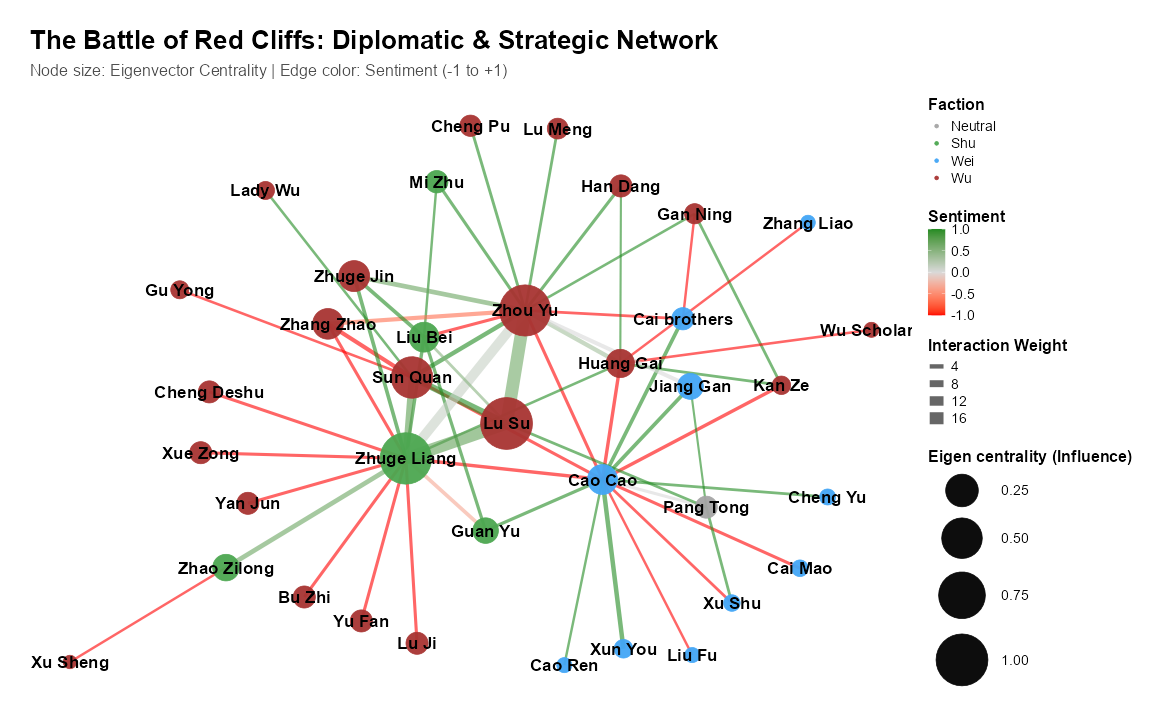
\includegraphics[width=0.9\linewidth]{RedCliffs_Network_graph.png}
        \caption{Person-person interaction network for \textbf{The Battle of Red Cliffs: Diplomatic and Strategic Network}. Node size represents eigenvector centrality, node colour represents faction, edge width represents interaction weight and edge colour represents sentiment }
        \label{fig:placeholder}
    \end{figure}

      

\subsection{Spatial GIS Analysis}
\label{sec:gis_methods}

Geographic analysis was conducted in QGIS, projecting narrative locations
onto a modern basemap  using approximate coordinate
assignments derived from cross-referencing the historical geography of the
Eastern Han / Three Kingdoms period.
Coordinate uncertainty was recorded as a categorical field
(High / Medium / Low confidence) and propagated into spatial aggregations.

Three spatial outputs were produced:
\begin{enumerate}[noitemsep]
  \item \textbf{Interaction heat map}: each person to place edge contributes a
        weighted point event; kernel density estimation reveals the spatial
        distribution of coalition activity.
        See \figref{fig:interaction_map}
  \item \textbf{Route reconstruction map}: character movement between
        successive locations is modelled as straight-line segments
        (geodesics), colour-coded by character, forming a trajectory overlay.
        See \figref{fig:spatial_gis}.
  \item \textbf{Timeline route visualisation}: movement segments are ordered
        chronologically by chapter section, allowing reading of spatial
        dynamics as narrative progresses.
        See \figref{fig:movement_timeline}.
\end{enumerate}
\begin{figure}[H]
  \centering
    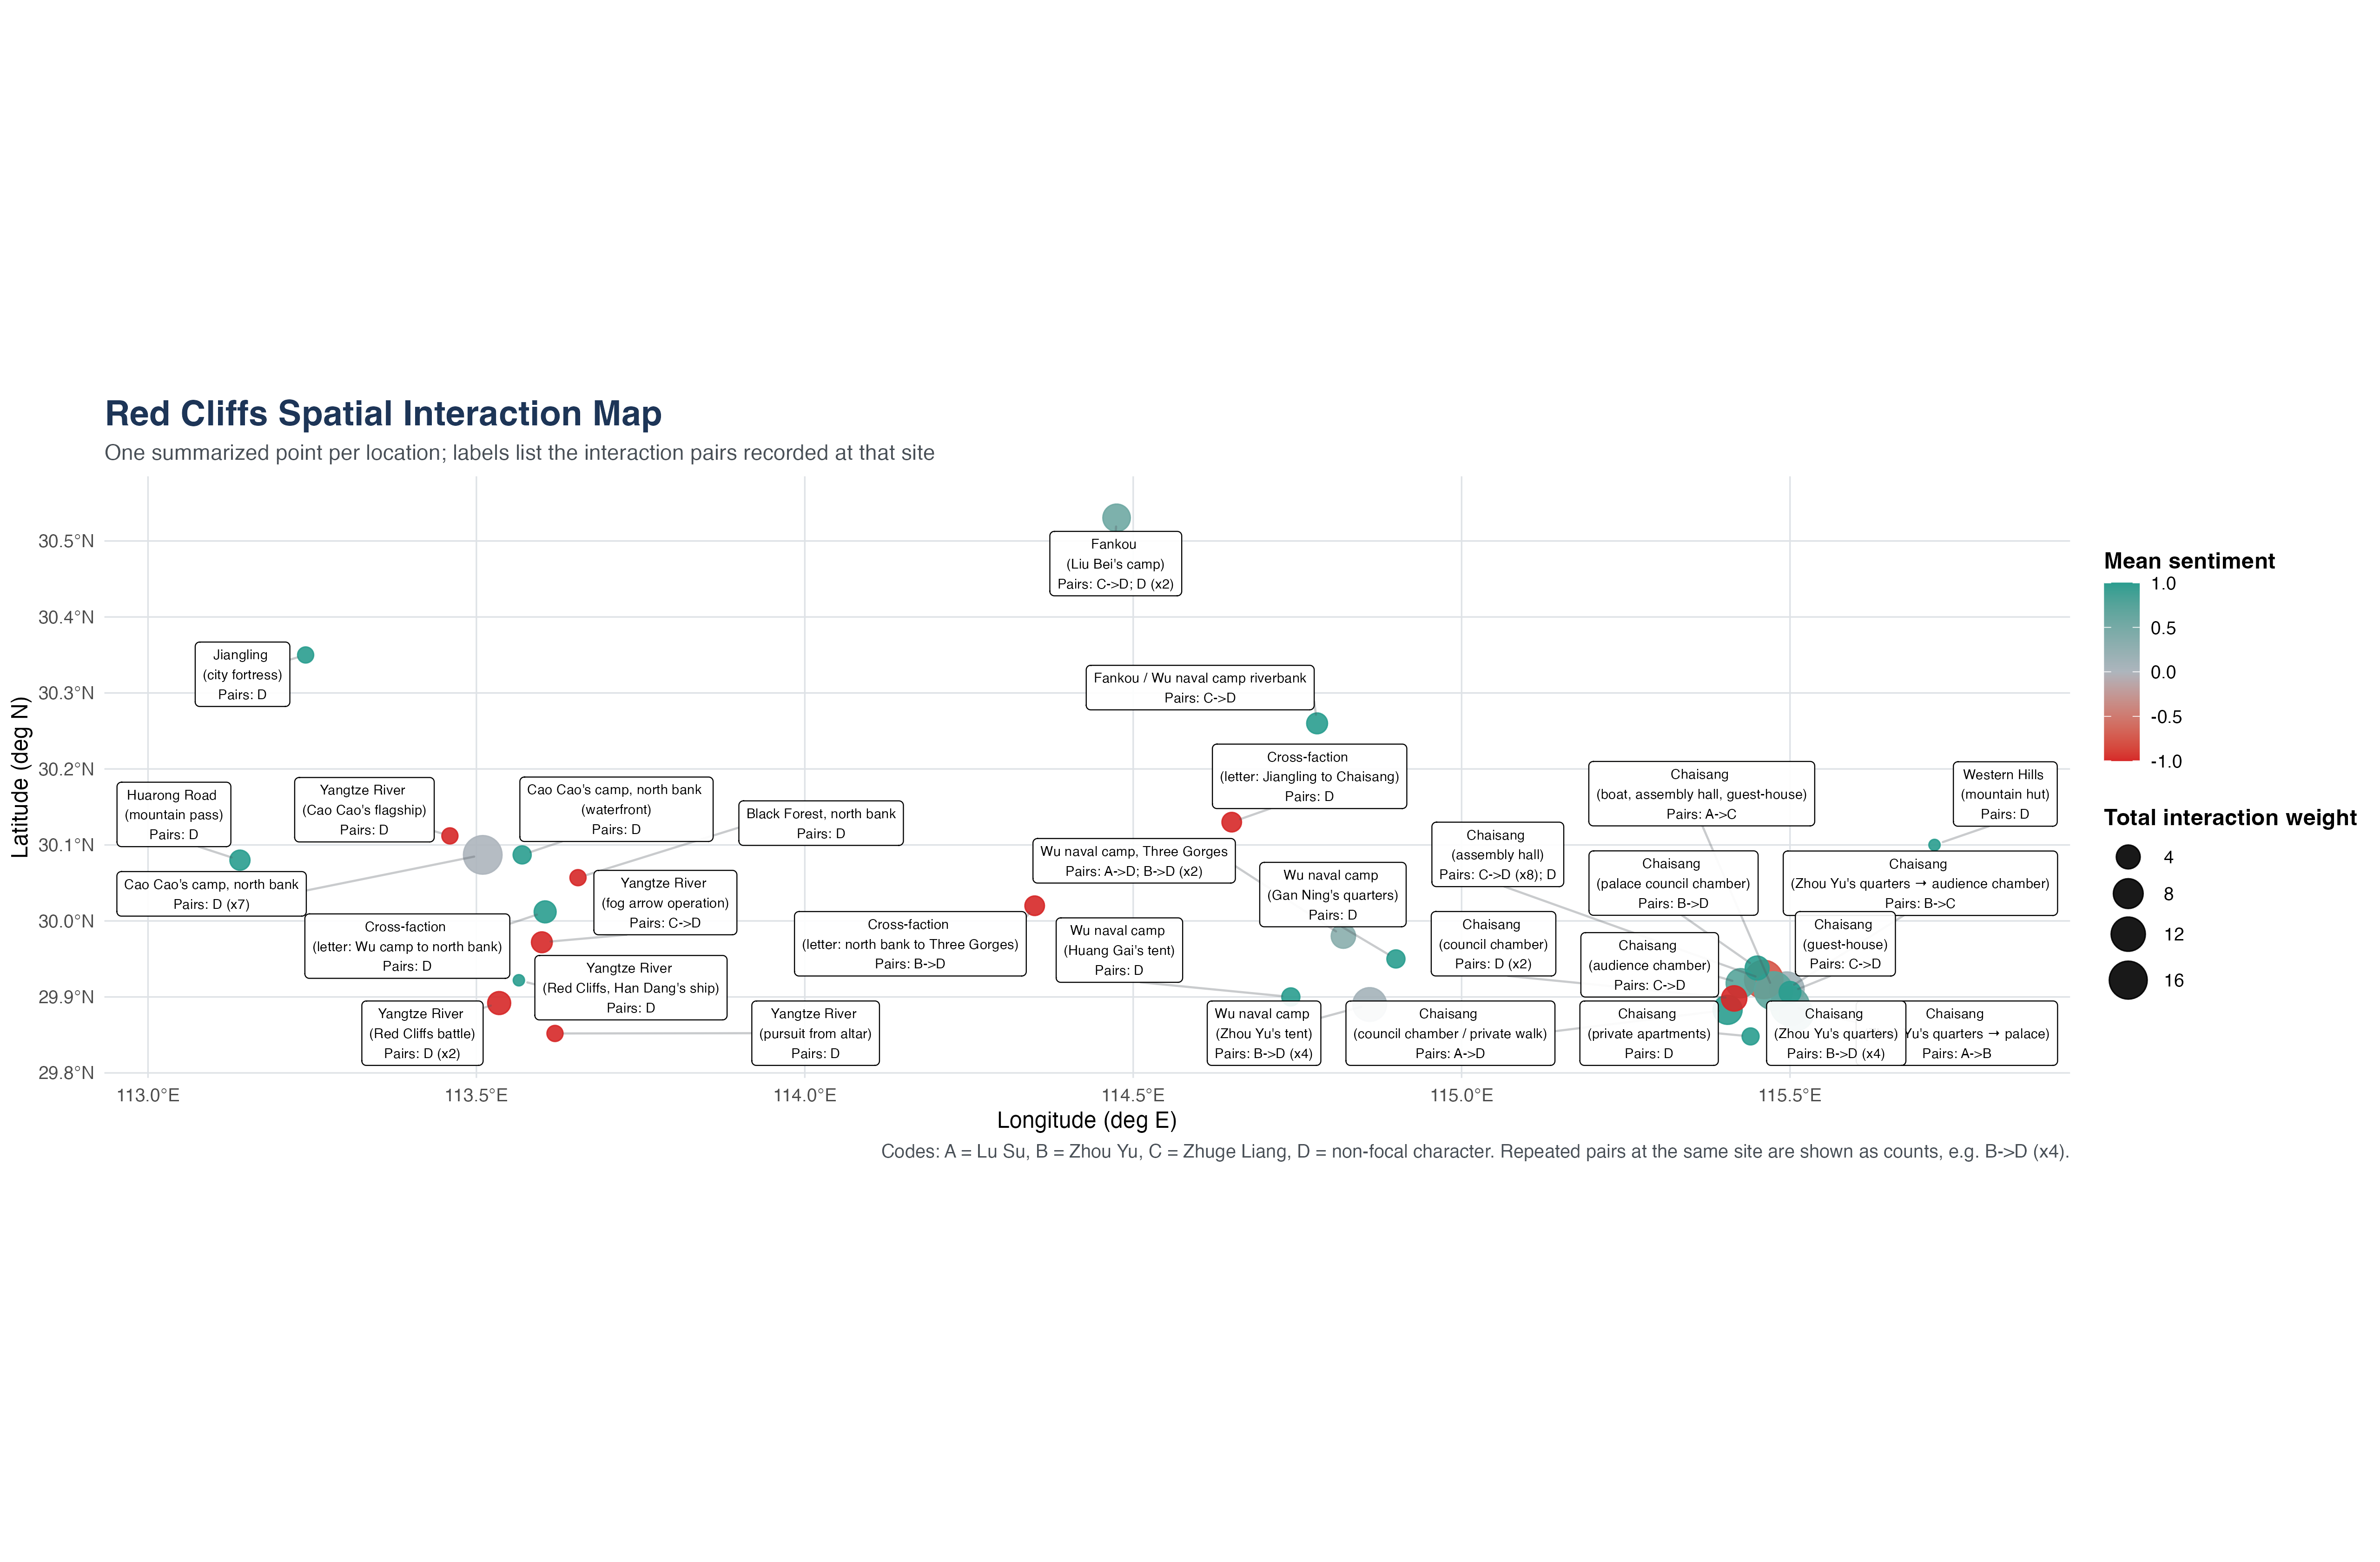
\includegraphics[width=\linewidth]{red_cliffs_spatial_proxy_map.png}
  \caption{GIS-based spatial interaction map for Chapters~43 through~50.
           Warmer regions indicate higher narrative activity density.
           The Yangtze River functions as both a geographic and
           political boundary in the narrative.}
  \label{fig:interaction_map}
\end{figure}

\begin{figure}[H]
  \centering
    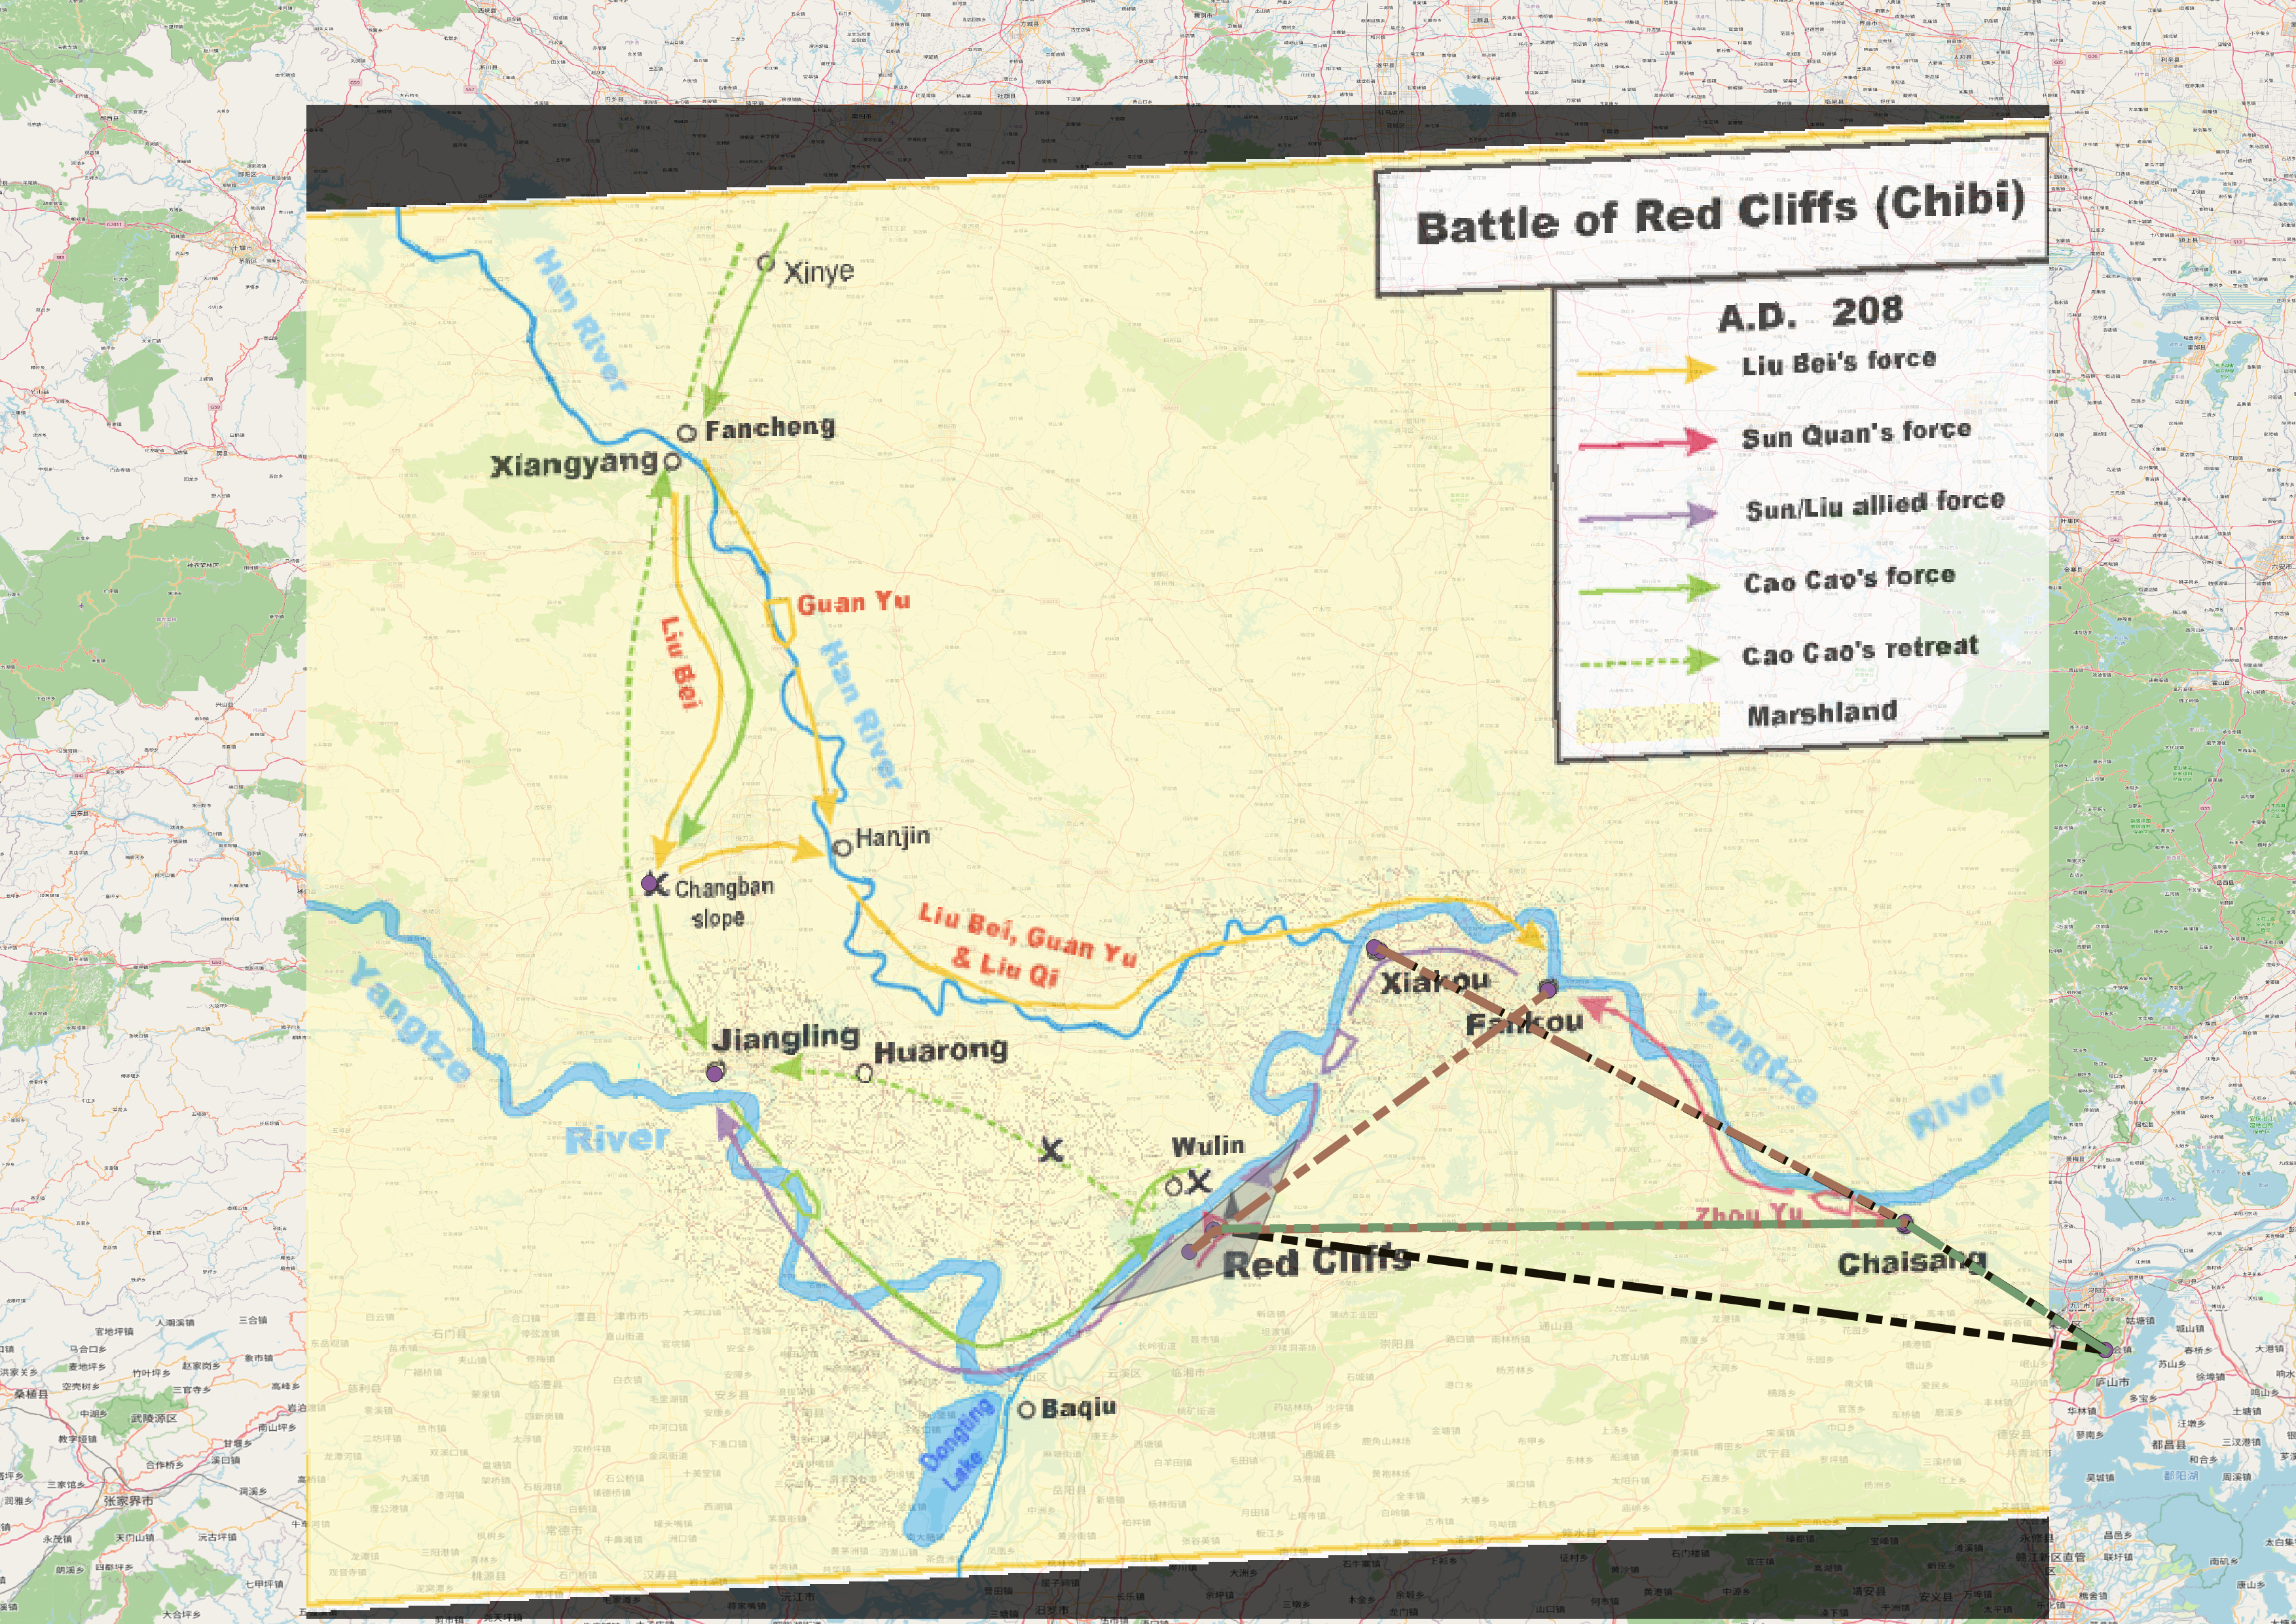
\includegraphics[width=0.9\linewidth]{Layout 3.png}
  \caption{QGIS layer on modern basemap}
  \label{fig:spatial_gis}
\end{figure}

\begin{figure}[H]
  \centering
  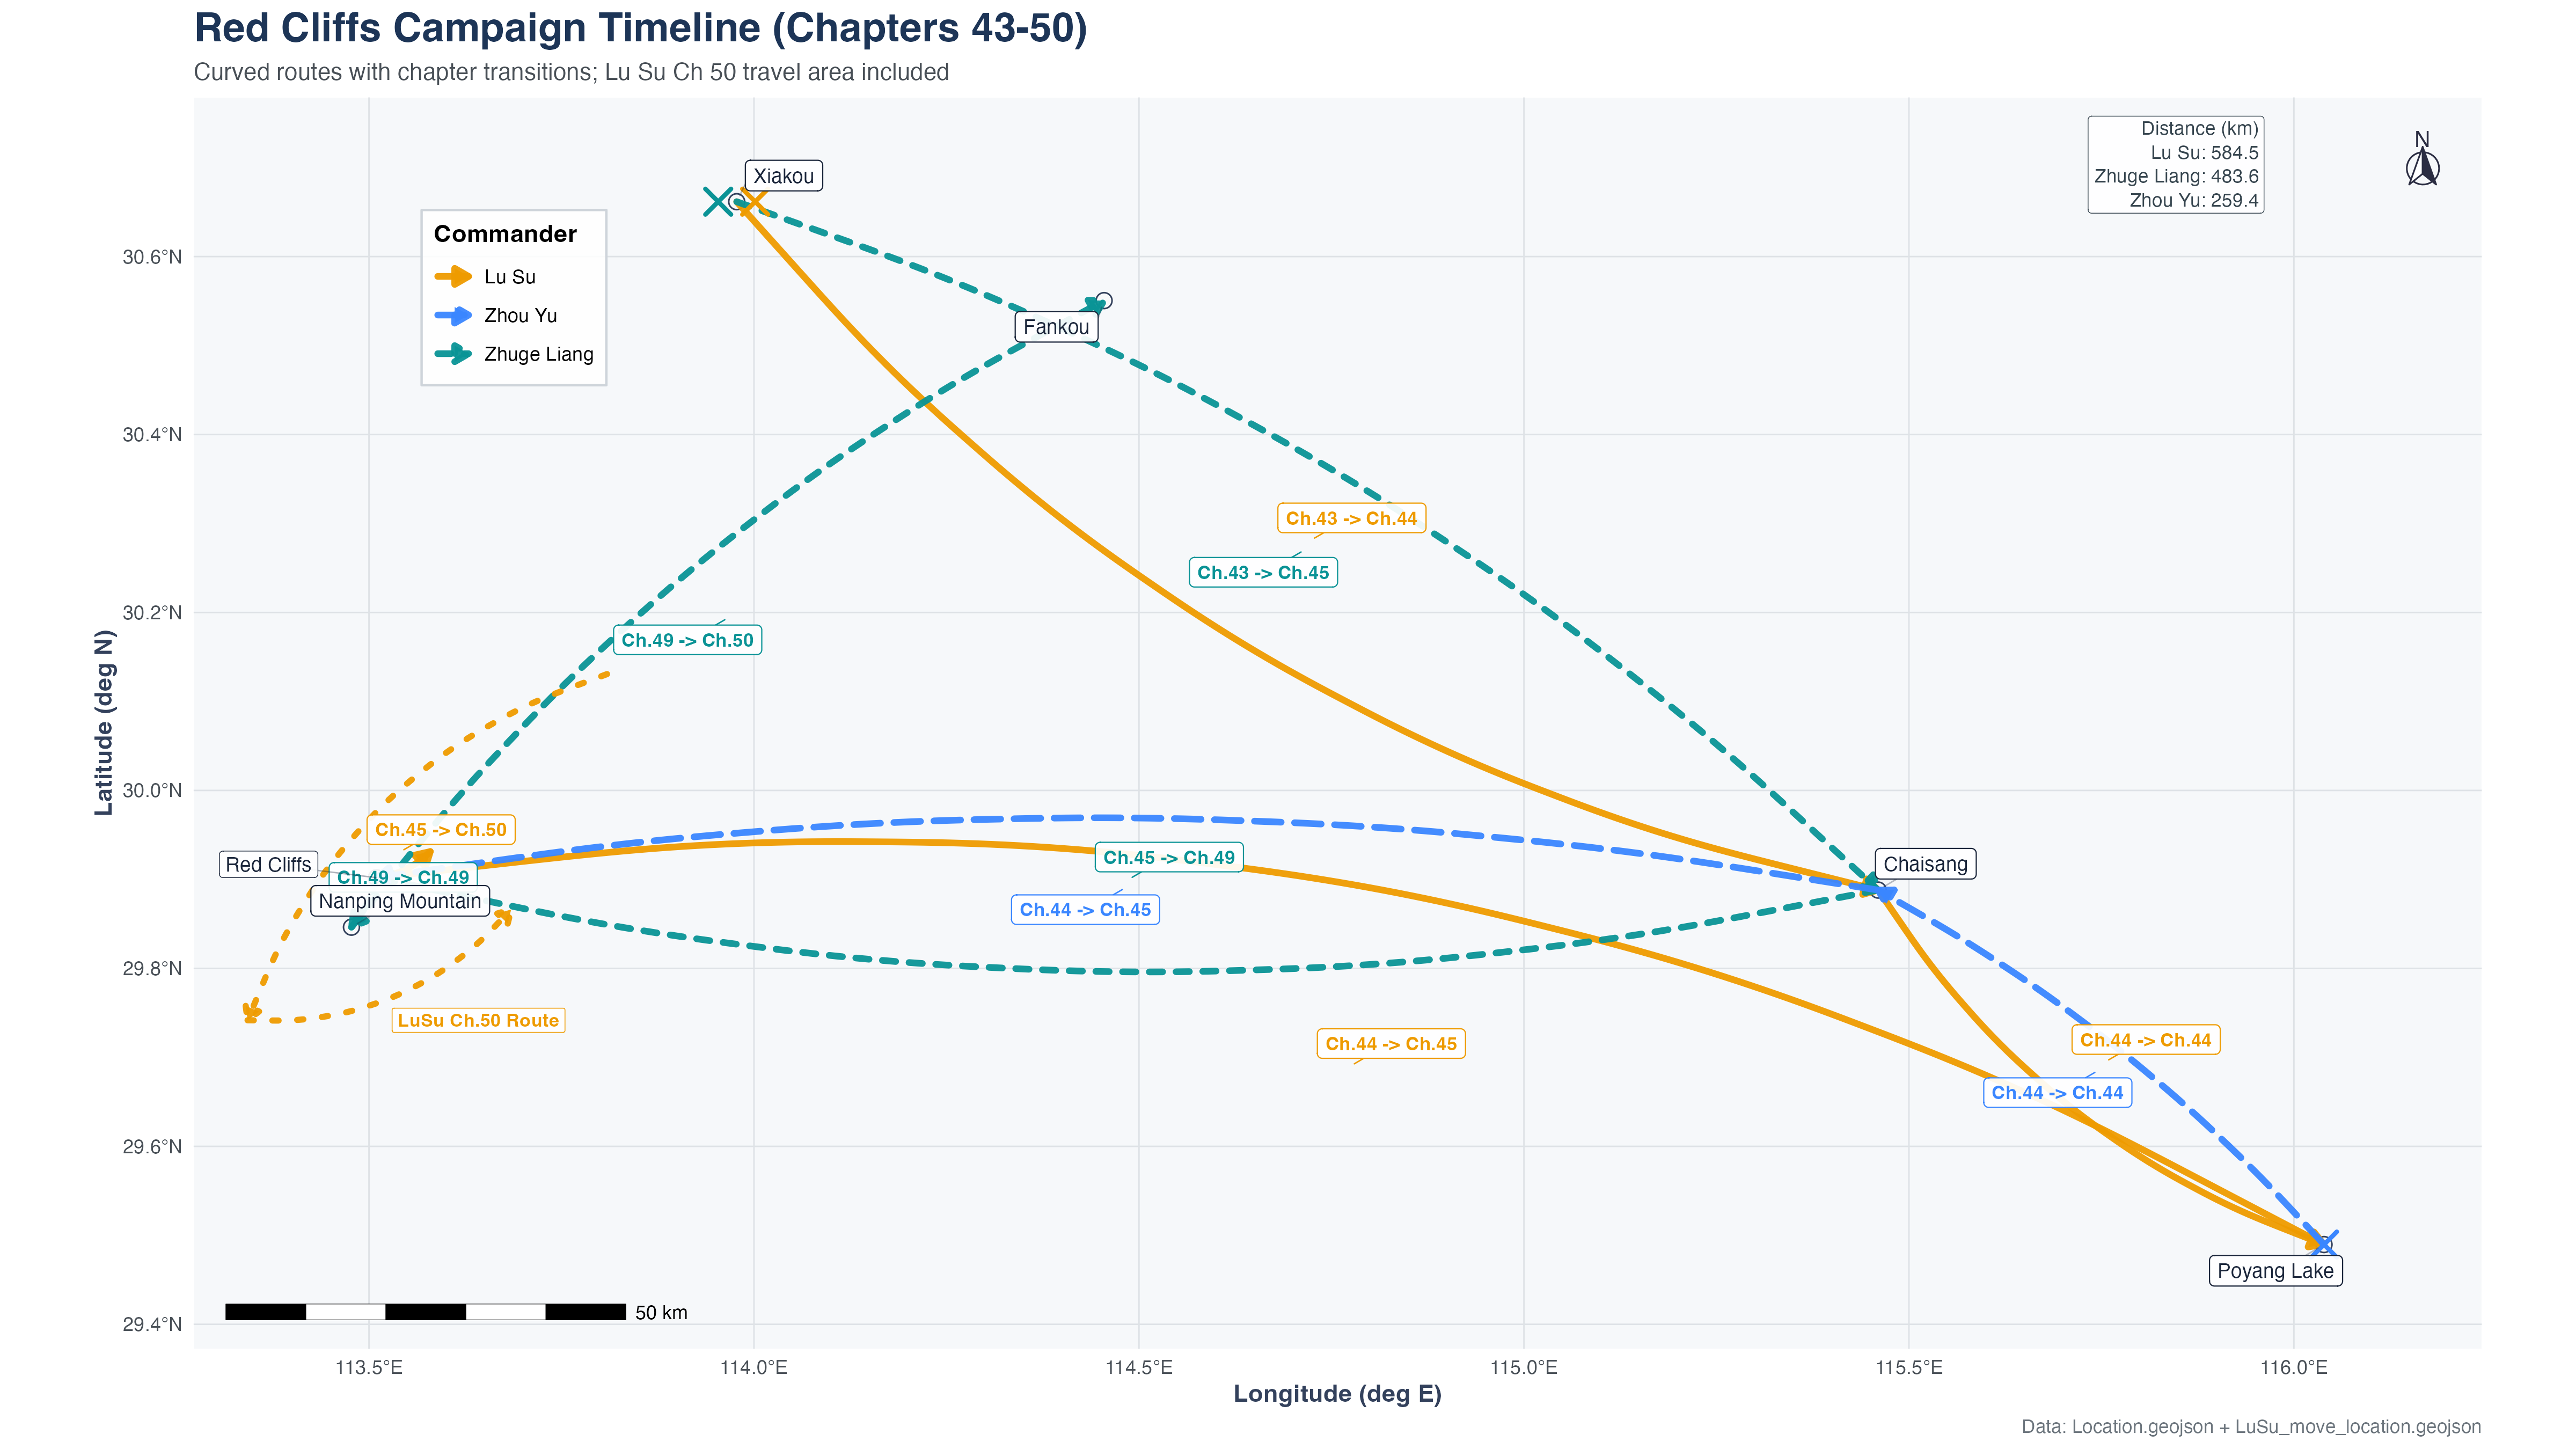
\includegraphics[width=\linewidth]{timeline_red_cliffs_professional.png}
  \caption{Timeline-based character movement route map.
           Lu Su's trajectory spans the greatest lateral distance,
           crossing the Wu and Shu spatial boundary multiple times.
           Zhou Yu remains anchored in Wu naval territory;
           Zhuge Liang exhibits long-range but episodic mobility.}
  \label{fig:movement_timeline}
\end{figure}

\subsection{R Code: Key Functions and Representative Snippets}
\label{sec:code}

The listings below are pseudocode-style summaries of the analysis pipeline.
Full scripts (network plot, route reconstruction, timeline map) are available
in the project repository.

\begin{lstlisting}[caption={Network construction and centrality (\texttt{tidygraph});
                            abbreviated pipeline.},
                   label={lst:network_build}]
# PSEUDOCODE: see repository for full script
library(tidyverse)
library(tidygraph)

nodes <- read_csv("Nodes_table_Red_Cliffs.csv")
edges <- read_csv("Edges_table_Red_Cliffs.csv")

person_edges <- edges %>%
  filter(Type == "Human interaction") %>%
  rename(from = Nodes_A, to = Nodes_B)

rc_graph <- tbl_graph(nodes, person_edges, directed = FALSE) %>%
  activate(nodes) %>%
  mutate(
    degree_score = centrality_degree(weights = Weight),
    eigen_score  = centrality_eigen(weights = Weight)
  )
# export centrality table; plot with ggraph (see prose below)
\end{lstlisting}

The network figure (Figure~\ref{fig:placeholder}) is produced with
\texttt{ggraph()} and a stress layout: node size encodes eigenvector
centrality, node colour faction, edge width interaction weight and edge
colour mean sentiment.

\begin{lstlisting}[caption={Map 1: interaction map (\texttt{sf} / \texttt{ggplot2});
                            abbreviated pipeline.},
                   label={lst:spatial_interaction}]
# PSEUDOCODE: see red_cliffs_centrality_analysis.R
library(tidyverse)
library(sf)
library(ggplot2)

df <- read_csv("red_cliffs_with_locations.csv")
# assign proxy lon/lat per Location_Name (resolve_proxy_coord)

spatial_df <- df %>%
  left_join(location_proxy, by = "Location_Name") %>%
  group_by(Location_Name, lon, lat) %>%
  summarise(total_weight = sum(Weight),
            mean_sentiment = mean(Sentiment), .groups = "drop")

pts_sf <- st_as_sf(spatial_df, coords = c("lon", "lat"), crs = 4326)

ggplot() +
  geom_sf(data = pts_sf, aes(size = total_weight, colour = mean_sentiment)) +
  coord_sf(expand = FALSE)
\end{lstlisting}

\begin{lstlisting}[caption={Map 2: route reconstruction (\texttt{sf})},
                   label={lst:spatial_routes}]
# PSEUDOCODE: see loading_example.R
library(sf)

loc <- st_read("Location.geojson", quiet = TRUE)

linestring_from_places <- function(place_sf, ordered_names) {
  m <- st_coordinates(place_sf[match(ordered_names, place_sf$name), ])
  st_sf(geometry = st_sfc(st_linestring(m[, 1:2]), crs = st_crs(place_sf)))
}

path_lusu  <- assemble_lusu_routes()   # shapefile or waypoint polyline
path_zhou  <- linestring_from_places(loc, c("Poyang_lake", "Chaisang", "RedCliffs"))
path_zhuge <- linestring_from_places(loc, c("Xiakou", "Chaisang", "RedCliffs", "Fankou"))

plot(st_geometry(loc), pch = 21, add = FALSE)
plot(st_geometry(path_lusu),  add = TRUE, col = "#e67e22", lwd = 2.8)
plot(st_geometry(path_zhou),  add = TRUE, col = "#1f77b4", lwd = 2.8)
plot(st_geometry(path_zhuge), add = TRUE, col = "#2ca02c", lwd = 2.8)
\end{lstlisting}

\begin{lstlisting}[caption={Map 3: timeline route map (\texttt{sf} / \texttt{ggplot2});
                            abbreviated pipeline.},
                   label={lst:spatial_timeline}]
# PSEUDOCODE: see new_example.R
library(sf)
library(ggplot2)
library(ggrepel)

loc <- st_read("Location.geojson", quiet = TRUE)
timeline <- data.frame(...)  # cols: track, chapter, place, stop_idx
# join place -> lon/lat; make_segments() -> one row per chapter leg

ggplot() +
  geom_sf(data = loc) +
  geom_curve(data = segments_df,
             aes(x, y, xend, yend, colour = track),
             arrow = arrow(type = "closed"), linewidth = 1.4) +
  geom_label_repel(data = chapter_labels, aes(label = chapter_label)) +
  coord_sf(xlim = c(bbox$xmin, bbox$xmax),
           ylim = c(bbox$ymin, bbox$ymax), expand = FALSE)
\end{lstlisting}

All three spatial outputs in \S\ref{sec:gis_methods} use WGS\,84 (EPSG:4326).
Map~1 aggregates interaction events to weighted points (\texttt{st\_as\_sf});
Map~2 connects ordered stops with \texttt{st\_linestring()}; Map~3 draws
chapter transitions with \texttt{geom\_curve()}. Full scripts are in the
project repository.

% ============================================================
\section{Results}
\label{sec:results}
% ============================================================

\subsection{Network Findings}
\label{sec:network_results}

\subsubsection{Centrality Divergence: Degree vs.\ Eigenvector}

Table~\ref{tab:centrality} presents the top-ten characters ranked by weighted
degree centrality; eigenvector scores are shown for comparison (highest score
held by Lu Su).

\begin{table}[H]
\centering
\caption{Top-ten character centrality scores,
         \booktitle{Romance of the Three Kingdoms}, Chapters~43 through~50.}
\label{tab:centrality}
\begin{tabularx}{0.82\textwidth}{l l c c c}
\toprule
\textbf{Rank} & \textbf{Character} & \textbf{Faction}
              & \textbf{Degree} & \textbf{Eigenvector} \\
\midrule
1  & Zhuge Liang & Shu     & 66.8 & 0.977 \\
2  & Zhou Yu     & Wu      & 63.3 & 0.965 \\
3  & Lu Su       & Wu      & 43.8 & \textbf{1.000} \\
4  & Cao Cao     & Wei     & 32.9 & 0.186 \\
5  & Sun Quan    & Wu      & 26.9 & 0.537 \\
6  & Liu Bei     & Shu     & 12.2 & 0.185 \\
7  & Huang Gai   & Wu      & 11.9 & 0.151 \\
8  & Zhuge Jin   & Wu      & 10.4 & 0.210 \\
9  & Zhang Zhao  & Wu      &  9.3 & 0.203 \\
10 & Guan Yu     & Shu     &  7.4 & 0.102 \\
\bottomrule
\end{tabularx}
\end{table}

The divergence is striking.
Zhuge Liang and Zhou Yu rank first and second in degree centrality,
reflecting their extensive narrative presence across the chapters.
Yet it is Lu Su who achieves the highest eigenvector centrality score (1.000),
indicating that his interaction partners are themselves among the most
centrally connected figures in the network.
Lu Su connects to Sun Quan, Zhou Yu, Liu Bei and Zhuge Liang (the four
most critical nodes in the coalition graph) and does so through
predominantly diplomatic-weight edges.
This positions him as a \emph{structural broker} in the Burtian sense:
a figure who occupies a bridging position across otherwise fragmented
subgraphs \autocite[Chapter~2]{burt2004brokerage}.

\subsubsection{Sentiment Topology of the Alliance}

The sentiment score of the Zhuge Liang and Zhou Yu edge is $-0.34$
(mildly hostile), making it one of the most negatively valenced
cross-factional dyads in the network.
Interactions between the two figures are consistently marked by
competitive display, mutual suspicion and veiled hostility: a
characterisation long acknowledged in literary criticism but here
quantified.

By contrast, Lu Su's edges present a distinctively positive sentiment
profile:
\begin{itemize}[noitemsep]
  \item Lu Su and Zhou Yu: $+0.72$ (strongly cooperative)
  \item Lu Su and Liu Bei: $+0.68$ (cooperative)
  \item Lu Su and Zhuge Liang: $+0.51$ (cooperative)
  \item Lu Su and Sun Quan: $+0.64$ (cooperative)
\end{itemize}

Lu Su is thus the only character who maintains cooperative sentiment
simultaneously with key Wu, Shu and de-facto neutral figures.
His positive valence with both Zhou Yu and Zhuge Liang, who cannot
sustain cooperation with each other, establishes him as an
\emph{affective buffer} whose presence is necessary to prevent
alliance collapse.

\subsubsection{Edge Weight Distribution}

A further structural asymmetry emerges when edge weights are disaggregated
by interaction type.
Approximately 71\% of Lu Su's total edge weight derives from Diplomatic
or Strategic interaction types (weight~$= 2.0$), compared with 54\% for
Zhuge Liang and 49\% for Zhou Yu.
The latter two figures devote a higher proportion of their interaction
budget to Persuasion and Command (weight~$= 1.0$), which, while narratively
visible, carry lower structural weight in coalition-maintenance terms.

\subsection{Spatial Findings}
\label{sec:spatial_results}

\subsubsection{Territorial Anchoring vs.\ Diplomatic Mobility}

The route reconstruction maps (\figref{fig:spatial_gis} and
\figref{fig:movement_timeline}) reveal three distinct spatial logics
operating within the same alliance:

\paragraph{Zhou Yu: Anchored Commander.}
Zhou Yu's movement is concentrated in Wu coastal and river-mouth territories:
Chaisang, Poyang Lake and the Red Cliffs naval staging zone.
His spatial footprint is deep within Wu territory.
He is a territorial commander whose authority is spatially bounded and
whose strategic legitimacy derives from control of the naval theatre.

\paragraph{Zhuge Liang: Long-Range but Episodic.}
Zhuge Liang covers the greatest single-journey distances, notably the
embassy crossing from Liu Bei's camp at Xiakou to Sun Quan's court at
Chaisang, but his spatial presence within Wu is \emph{episodic}:
he arrives, performs his diplomatic mission and withdraws.
He lacks territorial anchoring within the Wu spatial domain, which
limits his structural embeddedness in the coalition.

\paragraph{Lu Su: Mobile Diplomatic Infrastructure.}
Lu Su's trajectory is the most spatially continuous.
He travels between Liu Bei's camp, Sun Quan's court, Zhou Yu's military
headquarters and multiple deliberation sites, maintaining connection
across all spatial sub-zones of the coalition.
His route-distance across coalition-critical spatial transitions exceeds
that of both Zhuge Liang and Zhou Yu, and crucially his traversals
occur more evenly across the temporal span of the eight chapters,
suggesting sustained rather than punctual diplomatic labour.

\subsubsection{Chaisang as Spatial Centroid}

Kernel density estimation of person to place interaction events identifies
Chaisang as the spatial centroid of coalition formation activity:
it is the location with the highest aggregate interaction weight (score~=~4.7
on a relative 0 to 5 scale), serving as site for Sun Quan's deliberations,
Lu Su's briefings, Zhou Yu's military planning and Zhuge Liang's
persuasive oratory.
Its spatial position (at the confluence of Wu territory and the Yangtze
access corridor to Red Cliffs) makes it a logistical hub as well as a
political one.

\subsubsection{The Yangtze River as Narrative Boundary}

The Yangtze River functions in the spatial analysis as more than a
geographic feature.
In the interaction heat map, it serves as a visible boundary separating
Wu's high-density activity cluster from Cao Cao's isolated northern
encampment at Wulin.
The river marks a narrative logic of \emph{coalition cohesion} on its
southern bank versus \emph{strategic isolation} on its northern shore: a
spatial encoding of the very political asymmetry that made the fire-attack
strategy possible.

Red Cliffs itself, despite being the episode's climactic location, is not
a high-density interaction site in the person to place network: it is the
endpoint of converging trajectories, a zone of execution rather than
negotiation.
The coalition is \emph{formed} in Wu's interior (Chaisang); it is only
\emph{deployed} at Red Cliffs.
This spatial distinction challenges readings that treat the battle site as
the alliance's constitutive moment.

% ============================================================
\section{Discussion}
\label{sec:discussion}
% ============================================================

\subsection{Lu Su as Structural Broker}

Our network results converge on a theoretically coherent portrait of
Lu Su as a diplomatic broker in the classical sense described by
structural hole theory \autocite{burt2004brokerage}.
A structural hole exists when two otherwise disconnected (or poorly
connected) nodes depend on a third node for relay of information,
resources, or trust.
The Zhuge~Liang and Zhou~Yu negative-sentiment dyad constitutes precisely
such a configuration: two high-degree nodes who cannot effectively
coordinate without mediation.

Lu Su fills this structural hole not through accumulation of contacts
(degree centrality) but through the \emph{quality and positioning} of
his contacts (eigenvector centrality).
His uniquely high eigenvector score reflects that he is the only figure
in the network simultaneously well-connected to the principal agents of
both allied factions \emph{and} trusted by them.
This configuration makes him, in graph-theoretic terms, the node whose
removal would most dramatically degrade coalition connectivity: a
finding that corresponds to what historians have anecdotally identified
as Lu Su's ``indispensable'' role, but which the novel's narrative
presentation actively obscures through its rhetorical elevation of
Zhuge Liang.

\subsection{Fragile Alliance Theory}

Our integrated network-spatial analysis supports what we term a
\emph{fragile convergence} model of the Sun Liu alliance.
The coalition is not a merger of strategic wills but a temporary alignment
of separate political-spatial logics, held together by a single broker
whose removal would cause it to dissolve.

Three structural properties jointly constitute this fragility:

\begin{enumerate}
  \item \textbf{Sentiment brittleness at the core dyad.}
        The most narratively prominent cross-factional relationship
        (Zhuge Liang and Zhou Yu) is net-negative in sentiment.
        Alliance stability depends not on this dyad working well,
        but on Lu Su preventing it from failing catastrophically.

  \item \textbf{Spatial non-integration.}
        The coalition never achieves full spatial interpenetration.
        Wu and Shu characters occupy distinct territorial zones;
        their convergence at Red Cliffs is momentary, not structural.
        Once the battle concludes, the coalition geography immediately
        reasserts itself, as subsequent chapters confirm.

  \item \textbf{Asymmetric dependence.}
        Liu Bei and Zhuge Liang need Wu far more than Wu needs them.
        This asymmetry is encoded in the spatial mobility data:
        Shu figures travel into Wu territory; Wu figures do not
        travel into Shu.
        Lu Su's role is partly to manage the emotional and diplomatic
        consequences of this imbalance, which his consistently high
        cooperative sentiment scores reflect.
\end{enumerate}

This fragile-convergence reading has implications beyond the narrative.
The historical Battle of Red Cliffs was indeed followed by years of
territorial contention between Sun Quan and Liu Bei, during which
Lu Su famously worked to maintain the alliance against his own faction's
preference for reclaiming Jing Province.
Our computational reading of the novel's narrative structure thus
resonates with the political history it fictionalises.

\subsection{Integrating Network and Spatial Evidence}

The dual-method design yields interpretive dividends that neither approach
alone could produce.
Network analysis establishes \emph{who} is structurally indispensable;
spatial analysis explains \emph{why}: Lu Su's eigenvector centrality is
sustained by his continuous traversal of coalition geography, which allows
him to carry political intelligence, emotional reassurance and diplomatic
legitimacy across the spatial boundaries that separate his principals.

Zhuge Liang's long-range mobility could in principle achieve similar
effects, but his episodic presence within Wu territory means he cannot
sustain the ongoing relationship maintenance that coalition stability
requires.
Zhou Yu's deep territorial embeddedness gives him military authority
but precludes the inter-factional mobility that brokerage demands.
Only Lu Su moves continuously enough and widely enough to serve as the
coalition's diplomatic circulatory system.

\subsection{Narrative vs.\ Structural Visibility}

A meta-finding of this study is methodological: narrative prominence and
structural centrality diverge in systematic ways that DH methods can
surface.
The \booktitle{Romance of the Three Kingdoms} is constructed around a
rhetoric of strategic genius and martial virtue that centres Zhuge Liang
and Zhou Yu as its dramatic engines.
This rhetoric serves the novel's affective purposes: readers experience
the alliance through these figures' competing brilliances, but it
systematically displaces the unglamorous work of trust-building,
message-carrying and relationship-maintenance that Lu Su performs.

Moretti's argument that distant reading shifts attention from close analysis
of individual texts to patterns visible at the scale of the literary system
\autocite{moretti2005graphs} finds concrete illustration here.
A close reader of Chapters~43 through~50 might intuit Lu Su's importance;
the network analysis makes it precise, reproducible and theoretically
grounded.

% ============================================================
\section{Limitations}
\label{sec:limitations}
% ============================================================

\subsection{Narrative Bias in Sentiment Coding}

Sentiment scores are derived from textual events as rendered in English
translation.
Moss Roberts's translation, while scholarly, makes interpretive choices
that may inflate or deflate the hostility of particular interactions.
Moreover, the Cooperative / Neutral / Hostile trichotomy is a coarse
instrument: an interaction can be formally cooperative (an agreement is
reached) while containing undercurrents of mutual mistrust that the
coding scheme cannot capture.
Future work should explore finer-grained sentiment lexicons calibrated
to Classical Chinese rhetorical conventions.

\subsection{Uncertainty in Coordinate Mapping}

Assigning geographic coordinates to narrative locations involves
acknowledged imprecision.
While major locations (Chaisang, Red Cliffs, Xiakou) have well-attested
approximate positions, smaller sites named in the chapters may correspond
to multiple candidates in the historical geography, or may be entirely
fictional.
We recorded coordinate confidence levels, but the spatial analysis should
be understood as a model of relative spatial logic rather than an accurate
historical-geographic reconstruction.

\subsection{LLM Extraction Limitations}

Large-language-model extraction of character interactions, despite
multi-model validation and manual correction, introduces two systematic
biases.
First, LLMs tend to over-extract interactions involving characters who
receive heavy narratorial attention, which may inflate the degree
centrality of already prominent characters.
Second, indirect interactions (where a character acts on another's
behalf, or is the topic of discussion between third parties) are
inconsistently captured.
These limitations particularly affect the measurement of Lu Su's
influence, which is partly exerted through behind-the-scenes diplomatic
preparation that the novel narrates obliquely rather than directly.
Our manual correction stage addressed the most egregious cases but cannot
eliminate the pattern entirely.

\subsection{Single-Text Corpus}

Our analysis is based on one translation of one literary work.
Cross-linguistic validation (using the original classical Chinese text)
and cross-textual validation (against the historical \booktitle{Records
of the Three Kingdoms}) would strengthen the generalisability of the
findings.
\textcite{zhang2021complicating} provide a framework for such comparison
that future work could extend to the specific episode analysed here.

% ============================================================
\section{Conclusion}
\label{sec:conclusion}
% ============================================================

This paper has applied a hybrid Digital Humanities methodology, combining
LLM-assisted interaction extraction, network centrality analysis, and
GIS-based spatial mapping, applied to Chapters~43 through~50 of
\booktitle{Romance of the Three Kingdoms}.
Our principal finding is that Lu Su, not Zhuge Liang or Zhou Yu, functions
as the structural broker of the Sun Liu alliance.
His maximum eigenvector centrality score, his consistently cooperative
sentiment profile across all principal dyads and his unmatched spatial
continuity across coalition geography converge on a single interpretive
conclusion: the alliance at Red Cliffs is structurally dependent on one
character whose labour the novel systematically undervalues.

This \emph{fragile convergence} reading carries implications for how we
understand pre-modern Chinese alliance politics as novelistically encoded.
The \booktitle{Romance}'s rhetorical economy: its investment in martial
brilliance, strategic genius and the charismatic duel of Zhuge Liang
and Zhou Yu, renders invisible the unglamorous but essential work of
diplomatic maintenance.
Computational analysis makes that invisible labour visible, precise,
and theoretically articulable.

More broadly, this study demonstrates that Digital Humanities methods
bring genuine interpretive returns to classical Chinese fiction, a corpus
that has received less computational attention than European canonical
texts.
The hybrid pipeline developed here (controlled interaction extraction,
weighted sentiment-coded networks, and narrative-space GIS projection) is readily adaptable to other episodes, other novels and other
pre-modern narrative traditions.
Future work might extend the spatial analysis to the full \booktitle{Romance}
to examine how alliance geographies evolve across its 120 chapters, or
apply the brokerage-identification framework to other coalition episodes
in Chinese historical fiction.

\paragraph{Data and Code Availability.}
Interaction datasets, R analysis scripts, and QGIS layers are available at
\url{https://github.com/nhatminh37/HUMA_1678}.

% ============================================================
%  Bibliography
% ============================================================

\newpage
\printbibliography[title={References}]

\end{document}